%\chapter{Proponowane rozwiązanie}
\section{Proponowane rozwiązanie}
%\label{chapter-3}

\vspace{0.5cm}

\begin{comment}
Celem projektu było zaprojektowanie i skonstruowanie urządzenia umożliwiającego pomiar parametrów przetwornic napięciowych DC/DC, które przedstawione zostały w rozdziale \ref{chapter-2}.

Urządzenie takie powinno posiadać następujące właściwości:
\begin{itemize}
    \item Możliwość pomiaru sprawności przetwornic, regulacji napięcia wyjściowego, zakresu napięć wejściowych i prądów obciążenia.
    \item Modularność konstrukcji
    \item Możliwość dodania kolejnych modułów, umożliwiających wykonywanie innych pomiarów.
    \item Łatwość modyfikacji sprzętu i oprogramowania.    
    \item Niska cena w porównaniu do rozwiązań komercyjnych.
\end{itemize}

W celu spełnienia przedstawionych powyżej założeń, zaprojektowane urządzenie musi posiadać:
\begin{itemize}
    \item zintegrowany zasilacz regulowany
    \item zintegrowane obciążenie aktywne
    \item wbudowany kontroler, pozwalający na pracę bez konieczności podłączania do komputera, wyposażony w podstawowy interfejs użytkownika z wyświetlaczem
\end{itemize}

Elementy te zostały przedstawione na schemacie blokowym \ref{fig:schematBlokowy}.

\begin{figure}[h!]
    \begin{center}
        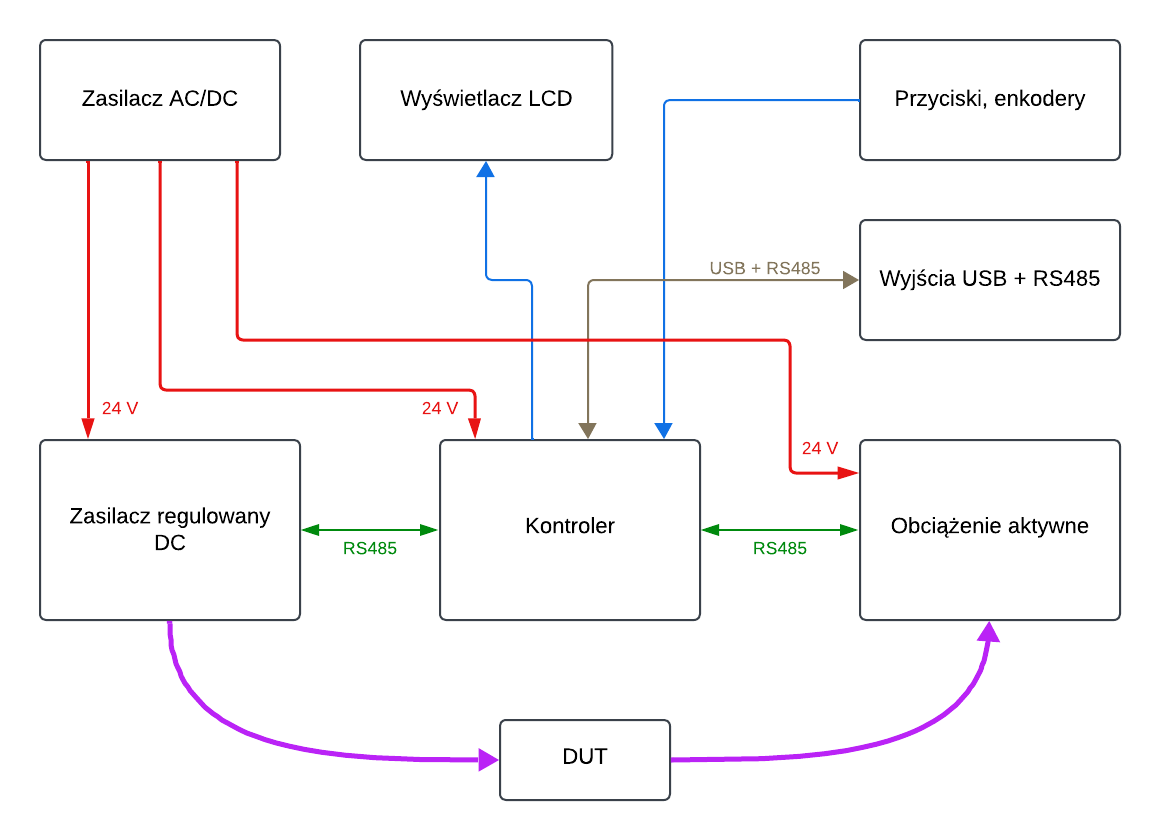
\includegraphics[width = 17cm]{images/schemat_blokowy.png}
        \caption{Schemat blokowy urządzenia.}
        \label{fig:schematBlokowy}
    \end{center}
\end{figure}

\end{comment}

Proponowane rozwiązanie zakłada projekt trzech modułów: kontrolera, obciążenia aktywnego i zasilacza regulowanego, 
które komunikują się między sobą przy pomocy odpowiedniego interfejsu.
Elementy te zostały przedstawione na schemacie blokowym \ref{fig:schematBlokowy}.
W celu umożliwienia użytkownikowi sterowania poszczególnymi modułami, urządzenie musi posiadać duży i czytelny wyświetlacz, a także panel frontowy z przyciskami i enkoderami.
Dodatkowe złącza USB oraz RS485 mają na celu umożliwienie sterowania poprzez komputer lub inne urządzenie laboratoryjne.
Za zasilanie wszystkich modułów odpowiada zasilacz, przekształcający napięcie sieciowe 230V AC na 24V DC, co pozwala uniknąć projektowania dedykowanych zasilaczy sieciowych dla każdego modułu.

Kolejnym ważnym aspektem jest zakres napięć i prądów, jakie dostarczyć należy do testowanej przetwornicy, oznaczonej na schemacie jako DUT
 (ang. \textit{Device Under Test}).
Zdecydowano się na zakres napięć wyjściowych 0-20 V i prąd do 2 A dla zasilacza regulowanego, jak również 0-20 V dla napięć wejściowych obciążenia aktywnego, z maksymalnym prądem 2A, co daje maksymalną wydzielaną moc na poziomie 40W.
Zdaniem autora, jest to zakres wystarczająco szeroki do testowania większości przetwornic, jakie stosowane są w wielu urządzeniach.
Zakłada to bowiem możliwość testowania przetwornic pracujących z napięciami: 3.3V, 5V, 9V, 12V, 15V, 20V, które znaleźć można np. w USB Power Delivery, a także
przetwarzających napięcie z akumulatorów LiIon, LiPo, lead-acid, LiFePO4.

Jak łatwo zauważyć, urządzenie takie umożliwia nie tylko pomiar parametrów przetwornic. Zasilacz regulowany oraz obciążenie aktywne mogą też być wykorzystywane oddzielnie,
zasilając inne urządzenia elektroniczne, dokonując pomiarów napięć i poboru prądu. 
Do mniej oczywistych zastosowań zaliczyć można pomiar pojemności baterii, mierząc ich ładowanie i rozładowanie, pomiar rezystancji przewodów, a co za tym idzie także ich długości, czy też automatyzacja pomiarów dokonywanych przez
inne sprzęty laboratoryjne, co można uzyskać podłączając je do wyprowadzeń kontrolera.

Znając już założenia projektu pod kątem elektrycznym, należy się skoncentrować nad aspektem mechanicznym urządzenia.
W celu uzyskania modularnej konstrukcji, która umożliwi dalszą rozbudowę, zdecydowano się ujednolicić konstrukcję poszczególnych modułów. 
Każdy z nich posiada PCB o wymiarach 150x100 mm. Wejściowe napięcie zasilające to 24V DC. Komunikacja natomiast odbywa się poprzez interfejs RS485. 

Szczegółowe rozwiązania układowe zostaly przedstawione w rozdziale \ref{chapter-4}, gdzie prezentowany jest zarówno projekt elektroniki, jak i obudowy i okablowania.

\begin{figure}[h!]
    \begin{center}
        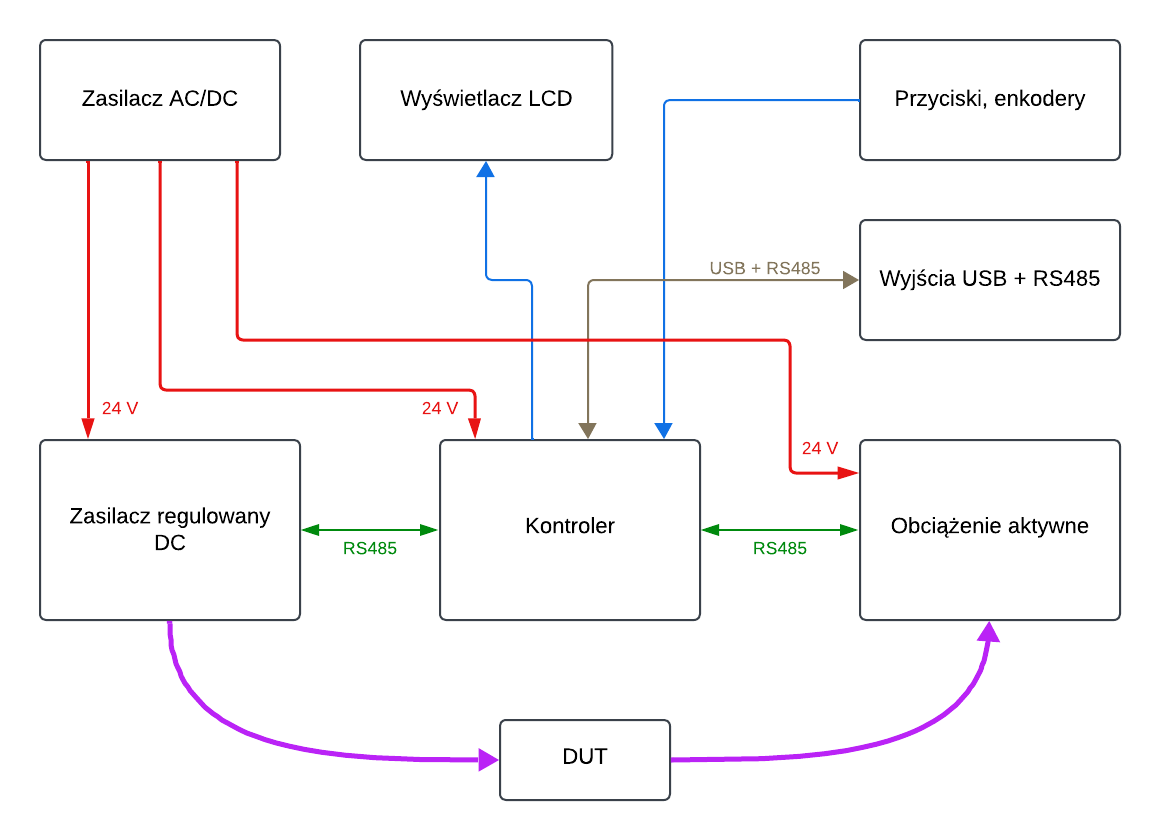
\includegraphics[width = 17cm]{images/schemat_blokowy.png}
        \caption{Schemat blokowy urządzenia.}
        \label{fig:schematBlokowy}
    \end{center}
\end{figure}








